\PassOptionsToPackage{unicode=true}{hyperref} % options for packages loaded elsewhere
\PassOptionsToPackage{hyphens}{url}
%
\documentclass[]{article}
\usepackage{lmodern}
\usepackage{amssymb,amsmath}
\usepackage{ifxetex,ifluatex}
\usepackage{fixltx2e} % provides \textsubscript
\ifnum 0\ifxetex 1\fi\ifluatex 1\fi=0 % if pdftex
  \usepackage[T1]{fontenc}
  \usepackage[utf8]{inputenc}
  \usepackage{textcomp} % provides euro and other symbols
\else % if luatex or xelatex
  \usepackage{unicode-math}
  \defaultfontfeatures{Ligatures=TeX,Scale=MatchLowercase}
\fi
% use upquote if available, for straight quotes in verbatim environments
\IfFileExists{upquote.sty}{\usepackage{upquote}}{}
% use microtype if available
\IfFileExists{microtype.sty}{%
\usepackage[]{microtype}
\UseMicrotypeSet[protrusion]{basicmath} % disable protrusion for tt fonts
}{}
\IfFileExists{parskip.sty}{%
\usepackage{parskip}
}{% else
\setlength{\parindent}{0pt}
\setlength{\parskip}{6pt plus 2pt minus 1pt}
}
\usepackage{hyperref}
\hypersetup{
            pdftitle={Multicollinearity},
            pdfauthor={Thiyanga S. Talagala},
            pdfborder={0 0 0},
            breaklinks=true}
\urlstyle{same}  % don't use monospace font for urls
\usepackage[margin=1in]{geometry}
\usepackage{color}
\usepackage{fancyvrb}
\newcommand{\VerbBar}{|}
\newcommand{\VERB}{\Verb[commandchars=\\\{\}]}
\DefineVerbatimEnvironment{Highlighting}{Verbatim}{commandchars=\\\{\}}
% Add ',fontsize=\small' for more characters per line
\usepackage{framed}
\definecolor{shadecolor}{RGB}{248,248,248}
\newenvironment{Shaded}{\begin{snugshade}}{\end{snugshade}}
\newcommand{\AlertTok}[1]{\textcolor[rgb]{0.94,0.16,0.16}{#1}}
\newcommand{\AnnotationTok}[1]{\textcolor[rgb]{0.56,0.35,0.01}{\textbf{\textit{#1}}}}
\newcommand{\AttributeTok}[1]{\textcolor[rgb]{0.77,0.63,0.00}{#1}}
\newcommand{\BaseNTok}[1]{\textcolor[rgb]{0.00,0.00,0.81}{#1}}
\newcommand{\BuiltInTok}[1]{#1}
\newcommand{\CharTok}[1]{\textcolor[rgb]{0.31,0.60,0.02}{#1}}
\newcommand{\CommentTok}[1]{\textcolor[rgb]{0.56,0.35,0.01}{\textit{#1}}}
\newcommand{\CommentVarTok}[1]{\textcolor[rgb]{0.56,0.35,0.01}{\textbf{\textit{#1}}}}
\newcommand{\ConstantTok}[1]{\textcolor[rgb]{0.00,0.00,0.00}{#1}}
\newcommand{\ControlFlowTok}[1]{\textcolor[rgb]{0.13,0.29,0.53}{\textbf{#1}}}
\newcommand{\DataTypeTok}[1]{\textcolor[rgb]{0.13,0.29,0.53}{#1}}
\newcommand{\DecValTok}[1]{\textcolor[rgb]{0.00,0.00,0.81}{#1}}
\newcommand{\DocumentationTok}[1]{\textcolor[rgb]{0.56,0.35,0.01}{\textbf{\textit{#1}}}}
\newcommand{\ErrorTok}[1]{\textcolor[rgb]{0.64,0.00,0.00}{\textbf{#1}}}
\newcommand{\ExtensionTok}[1]{#1}
\newcommand{\FloatTok}[1]{\textcolor[rgb]{0.00,0.00,0.81}{#1}}
\newcommand{\FunctionTok}[1]{\textcolor[rgb]{0.00,0.00,0.00}{#1}}
\newcommand{\ImportTok}[1]{#1}
\newcommand{\InformationTok}[1]{\textcolor[rgb]{0.56,0.35,0.01}{\textbf{\textit{#1}}}}
\newcommand{\KeywordTok}[1]{\textcolor[rgb]{0.13,0.29,0.53}{\textbf{#1}}}
\newcommand{\NormalTok}[1]{#1}
\newcommand{\OperatorTok}[1]{\textcolor[rgb]{0.81,0.36,0.00}{\textbf{#1}}}
\newcommand{\OtherTok}[1]{\textcolor[rgb]{0.56,0.35,0.01}{#1}}
\newcommand{\PreprocessorTok}[1]{\textcolor[rgb]{0.56,0.35,0.01}{\textit{#1}}}
\newcommand{\RegionMarkerTok}[1]{#1}
\newcommand{\SpecialCharTok}[1]{\textcolor[rgb]{0.00,0.00,0.00}{#1}}
\newcommand{\SpecialStringTok}[1]{\textcolor[rgb]{0.31,0.60,0.02}{#1}}
\newcommand{\StringTok}[1]{\textcolor[rgb]{0.31,0.60,0.02}{#1}}
\newcommand{\VariableTok}[1]{\textcolor[rgb]{0.00,0.00,0.00}{#1}}
\newcommand{\VerbatimStringTok}[1]{\textcolor[rgb]{0.31,0.60,0.02}{#1}}
\newcommand{\WarningTok}[1]{\textcolor[rgb]{0.56,0.35,0.01}{\textbf{\textit{#1}}}}
\usepackage{graphicx,grffile}
\makeatletter
\def\maxwidth{\ifdim\Gin@nat@width>\linewidth\linewidth\else\Gin@nat@width\fi}
\def\maxheight{\ifdim\Gin@nat@height>\textheight\textheight\else\Gin@nat@height\fi}
\makeatother
% Scale images if necessary, so that they will not overflow the page
% margins by default, and it is still possible to overwrite the defaults
% using explicit options in \includegraphics[width, height, ...]{}
\setkeys{Gin}{width=\maxwidth,height=\maxheight,keepaspectratio}
\setlength{\emergencystretch}{3em}  % prevent overfull lines
\providecommand{\tightlist}{%
  \setlength{\itemsep}{0pt}\setlength{\parskip}{0pt}}
\setcounter{secnumdepth}{0}
% Redefines (sub)paragraphs to behave more like sections
\ifx\paragraph\undefined\else
\let\oldparagraph\paragraph
\renewcommand{\paragraph}[1]{\oldparagraph{#1}\mbox{}}
\fi
\ifx\subparagraph\undefined\else
\let\oldsubparagraph\subparagraph
\renewcommand{\subparagraph}[1]{\oldsubparagraph{#1}\mbox{}}
\fi

% set default figure placement to htbp
\makeatletter
\def\fps@figure{htbp}
\makeatother


\title{Multicollinearity}
\author{Thiyanga S. Talagala}
\date{2020-12-05 (live zoom)}

\begin{document}
\maketitle

\hypertarget{introduction}{%
\subsection{1. Introduction}\label{introduction}}

Multicollinearity refers to a situation in which two or more
\textbf{explanatory variables} in a multiple regression model are highly
linearly related.

\hypertarget{data}{%
\subsection{2. Data}\label{data}}

\begin{Shaded}
\begin{Highlighting}[]
\KeywordTok{library}\NormalTok{(readr)}
\NormalTok{bloodpressure <-}\StringTok{ }\KeywordTok{read_csv}\NormalTok{(}\StringTok{"bloodpressure.csv"}\NormalTok{)}
\NormalTok{bloodpressure}
\end{Highlighting}
\end{Shaded}

\begin{verbatim}
# A tibble: 20 x 9
      X1    Pt    BP   Age Weight   BSA   Dur Pulse Stress
   <dbl> <dbl> <dbl> <dbl>  <dbl> <dbl> <dbl> <dbl>  <dbl>
 1     1     1   105    47   85.4  1.75   5.1    63     33
 2     2     2   115    49   94.2  2.1    3.8    70     14
 3     3     3   116    49   95.3  1.98   8.2    72     10
 4     4     4   117    50   94.7  2.01   5.8    73     99
 5     5     5   112    51   89.4  1.89   7      72     95
 6     6     6   121    48   99.5  2.25   9.3    71     10
 7     7     7   121    49   99.8  2.25   2.5    69     42
 8     8     8   110    47   90.9  1.9    6.2    66      8
 9     9     9   110    49   89.2  1.83   7.1    69     62
10    10    10   114    48   92.7  2.07   5.6    64     35
11    11    11   114    47   94.4  2.07   5.3    74     90
12    12    12   115    49   94.1  1.98   5.6    71     21
13    13    13   114    50   91.6  2.05  10.2    68     47
14    14    14   106    45   87.1  1.92   5.6    67     80
15    15    15   125    52  101.   2.19  10      76     98
16    16    16   114    46   94.5  1.98   7.4    69     95
17    17    17   106    46   87    1.87   3.6    62     18
18    18    18   113    46   94.5  1.9    4.3    70     12
19    19    19   110    48   90.5  1.88   9      71     99
20    20    20   122    56   95.7  2.09   7      75     99
\end{verbatim}

\hypertarget{variable-description}{%
\subsubsection{2.1 Variable description}\label{variable-description}}

\begin{enumerate}
\def\labelenumi{\arabic{enumi}.}
\item
  \(Y\): BP (blood pressure, in mmHg)
\item
  \(X_1\): Age (in years)
\item
  \(X_2\): Weight (in kg)
\item
  \(X_3\): BSA (body surface area, in sq m)
\item
  \(X_4\): Dur (duration of hypertension)
\item
  \(X_5\): Pulse (basal pulse)
\item
  \(X_6\): Stress (stress index)
\end{enumerate}

\hypertarget{how-to-detect-multicollinearity}{%
\subsection{3. How to detect
multicollinearity?}\label{how-to-detect-multicollinearity}}

\begin{enumerate}
\def\labelenumi{\arabic{enumi}.}
\tightlist
\item
  Correlation matrix and scatterplot matrix
\end{enumerate}

This is limiting. It is possible that the pairwise correlations between
variables are small, but a linear dependence exists among three or even
more variables in the dataset. Hence, we use \textbf{variance inflation
factors (VIF)} to detect multicollinearity.

\begin{Shaded}
\begin{Highlighting}[]
\KeywordTok{library}\NormalTok{(GGally)}
\KeywordTok{ggpairs}\NormalTok{(bloodpressure[, }\OperatorTok{-}\KeywordTok{c}\NormalTok{(}\DecValTok{1}\NormalTok{, }\DecValTok{2}\NormalTok{)])}
\end{Highlighting}
\end{Shaded}

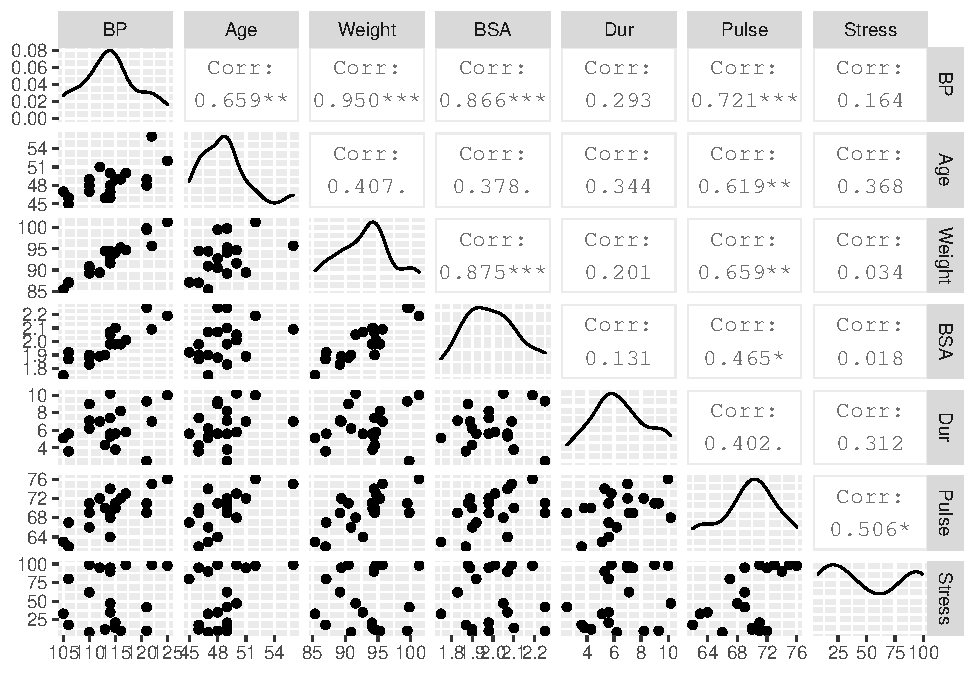
\includegraphics{regression13_files/figure-latex/unnamed-chunk-2-1.pdf}

\begin{enumerate}
\def\labelenumi{\arabic{enumi}.}
\setcounter{enumi}{1}
\tightlist
\item
  Variance Inflation Factors (VIF)
\end{enumerate}

Variance inflation factor for \(j^{th}\) variable

\[VIF_j = \frac{1}{1-R^2_j}\]

where \(R^2_j\) is the \(R^2\) value obtained by regressing the
\(j^{th}\) predictor on the remaining predictors.

\begin{Shaded}
\begin{Highlighting}[]
\KeywordTok{library}\NormalTok{(broom)}
\NormalTok{bp <-}\StringTok{ }\KeywordTok{lm}\NormalTok{(BP }\OperatorTok{~}\StringTok{ }\NormalTok{Age }\OperatorTok{+}\StringTok{ }\NormalTok{Weight }\OperatorTok{+}\StringTok{ }\NormalTok{BSA }\OperatorTok{+}\StringTok{ }\NormalTok{Dur }\OperatorTok{+}\StringTok{ }\NormalTok{Pulse }\OperatorTok{+}\StringTok{ }\NormalTok{Stress, }\DataTypeTok{data=}\NormalTok{bloodpressure)}
\NormalTok{bp}
\end{Highlighting}
\end{Shaded}

\begin{verbatim}

Call:
lm(formula = BP ~ Age + Weight + BSA + Dur + Pulse + Stress, 
    data = bloodpressure)

Coefficients:
(Intercept)          Age       Weight          BSA          Dur        Pulse  
 -12.870476     0.703259     0.969920     3.776491     0.068383    -0.084485  
     Stress  
   0.005572  
\end{verbatim}

\begin{Shaded}
\begin{Highlighting}[]
\KeywordTok{summary}\NormalTok{(bp)}
\end{Highlighting}
\end{Shaded}

\begin{verbatim}

Call:
lm(formula = BP ~ Age + Weight + BSA + Dur + Pulse + Stress, 
    data = bloodpressure)

Residuals:
     Min       1Q   Median       3Q      Max 
-0.93213 -0.11314  0.03064  0.21834  0.48454 

Coefficients:
              Estimate Std. Error t value Pr(>|t|)    
(Intercept) -12.870476   2.556650  -5.034 0.000229 ***
Age           0.703259   0.049606  14.177 2.76e-09 ***
Weight        0.969920   0.063108  15.369 1.02e-09 ***
BSA           3.776491   1.580151   2.390 0.032694 *  
Dur           0.068383   0.048441   1.412 0.181534    
Pulse        -0.084485   0.051609  -1.637 0.125594    
Stress        0.005572   0.003412   1.633 0.126491    
---
Signif. codes:  0 '***' 0.001 '**' 0.01 '*' 0.05 '.' 0.1 ' ' 1

Residual standard error: 0.4072 on 13 degrees of freedom
Multiple R-squared:  0.9962,    Adjusted R-squared:  0.9944 
F-statistic: 560.6 on 6 and 13 DF,  p-value: 6.395e-15
\end{verbatim}

\hypertarget{calculate-vif}{%
\subsection{4. Calculate VIF}\label{calculate-vif}}

\begin{Shaded}
\begin{Highlighting}[]
\KeywordTok{library}\NormalTok{(car)}
\KeywordTok{vif}\NormalTok{(bp)}
\end{Highlighting}
\end{Shaded}

\begin{verbatim}
     Age   Weight      BSA      Dur    Pulse   Stress 
1.762807 8.417035 5.328751 1.237309 4.413575 1.834845 
\end{verbatim}

\hypertarget{illustration-of-the-output-for-weight-variable}{%
\subsection{5. Illustration of the output for weight
variable}\label{illustration-of-the-output-for-weight-variable}}

Build a regression model taking \emph{weight} as the dependent variable
and remaining \texttt{x} variables as the independent variables.

\begin{Shaded}
\begin{Highlighting}[]
\NormalTok{weight <-}\StringTok{ }\KeywordTok{lm}\NormalTok{(Weight }\OperatorTok{~}\StringTok{ }\NormalTok{Age  }\OperatorTok{+}\StringTok{ }\NormalTok{BSA }\OperatorTok{+}\StringTok{ }\NormalTok{Dur }\OperatorTok{+}\StringTok{ }\NormalTok{Pulse }\OperatorTok{+}\StringTok{ }\NormalTok{Stress, }\DataTypeTok{data=}\NormalTok{bloodpressure)}
\NormalTok{weight}
\end{Highlighting}
\end{Shaded}

\begin{verbatim}

Call:
lm(formula = Weight ~ Age + BSA + Dur + Pulse + Stress, data = bloodpressure)

Coefficients:
(Intercept)          Age          BSA          Dur        Pulse       Stress  
  19.674438    -0.144643    21.421654     0.008696     0.557697    -0.022997  
\end{verbatim}

\begin{Shaded}
\begin{Highlighting}[]
\KeywordTok{summary}\NormalTok{(weight)}
\end{Highlighting}
\end{Shaded}

\begin{verbatim}

Call:
lm(formula = Weight ~ Age + BSA + Dur + Pulse + Stress, data = bloodpressure)

Residuals:
    Min      1Q  Median      3Q     Max 
-2.7697 -1.0120  0.1960  0.6955  2.7035 

Coefficients:
             Estimate Std. Error t value Pr(>|t|)    
(Intercept) 19.674438   9.464742   2.079  0.05651 .  
Age         -0.144643   0.206491  -0.700  0.49510    
BSA         21.421654   3.464586   6.183 2.38e-05 ***
Dur          0.008696   0.205134   0.042  0.96678    
Pulse        0.557697   0.159853   3.489  0.00361 ** 
Stress      -0.022997   0.013079  -1.758  0.10052    
---
Signif. codes:  0 '***' 0.001 '**' 0.01 '*' 0.05 '.' 0.1 ' ' 1

Residual standard error: 1.725 on 14 degrees of freedom
Multiple R-squared:  0.8812,    Adjusted R-squared:  0.8388 
F-statistic: 20.77 on 5 and 14 DF,  p-value: 5.046e-06
\end{verbatim}

\[VIF_weight = \frac{1}{1-R^2_weight} = \frac{1}{1-0.8812} = 8.42\]

\textbf{VIFs exceeding 4 indicates high multicollinearity while VIFs
exceeding 10 are considered evidence of serious multicollinearity
requiring correction.}

\hypertarget{what-to-do-now}{%
\subsection{6. What to do now?}\label{what-to-do-now}}

One solution is to remove some of the variables with high VIF. Variables
\texttt{Weight}, \texttt{BSA} and \texttt{Pulse} have high VIF values.
If we review the pairwise correlations again, we can see \texttt{Weight}
and \texttt{BSA} are highly correlated. We can choose to remove either
predictor from the model.

Which one to remove? In-class discussion.

\begin{Shaded}
\begin{Highlighting}[]
\KeywordTok{library}\NormalTok{(GGally)}
\KeywordTok{ggpairs}\NormalTok{(bloodpressure[, }\OperatorTok{-}\KeywordTok{c}\NormalTok{(}\DecValTok{1}\NormalTok{, }\DecValTok{2}\NormalTok{)])}
\end{Highlighting}
\end{Shaded}

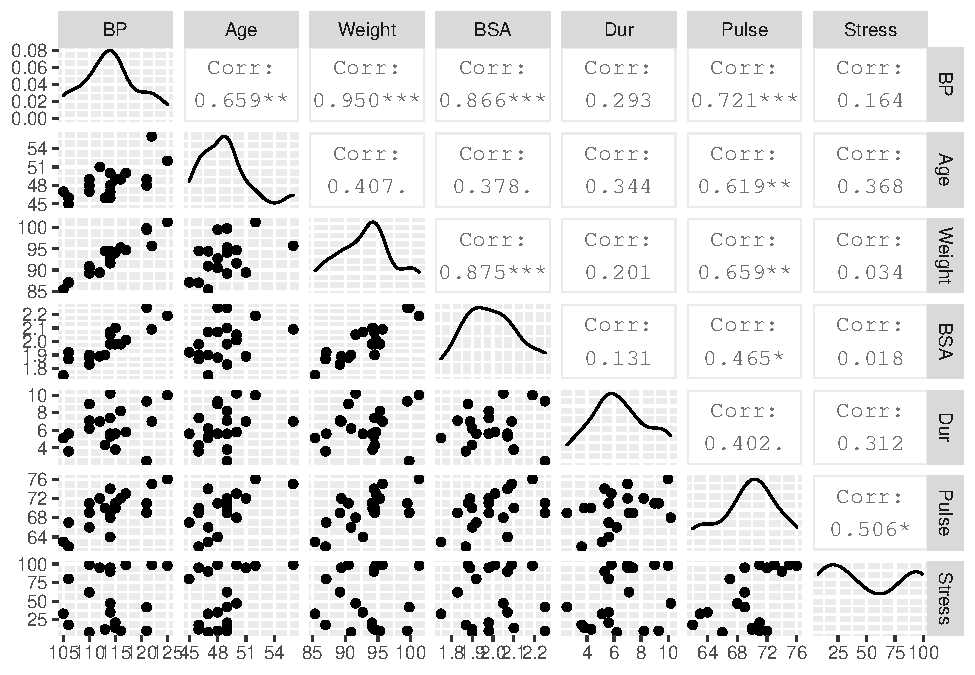
\includegraphics{regression13_files/figure-latex/unnamed-chunk-6-1.pdf}

\newpage

\hypertarget{new-model-without-pulse-and-bsa}{%
\subsection{\texorpdfstring{New model without \texttt{Pulse} and
\texttt{BSA}}{New model without Pulse and BSA}}\label{new-model-without-pulse-and-bsa}}

\begin{Shaded}
\begin{Highlighting}[]
\KeywordTok{library}\NormalTok{(broom)}
\NormalTok{bp2 <-}\StringTok{ }\KeywordTok{lm}\NormalTok{(BP }\OperatorTok{~}\StringTok{ }\NormalTok{Age }\OperatorTok{+}\StringTok{ }\NormalTok{Weight  }\OperatorTok{+}\StringTok{ }\NormalTok{Dur  }\OperatorTok{+}\StringTok{ }\NormalTok{Stress, }\DataTypeTok{data=}\NormalTok{bloodpressure)}
\NormalTok{bp2}
\end{Highlighting}
\end{Shaded}

\begin{verbatim}

Call:
lm(formula = BP ~ Age + Weight + Dur + Stress, data = bloodpressure)

Coefficients:
(Intercept)          Age       Weight          Dur       Stress  
 -15.869829     0.683741     1.034128     0.039889     0.002184  
\end{verbatim}

\begin{Shaded}
\begin{Highlighting}[]
\KeywordTok{summary}\NormalTok{(bp2)}
\end{Highlighting}
\end{Shaded}

\begin{verbatim}

Call:
lm(formula = BP ~ Age + Weight + Dur + Stress, data = bloodpressure)

Residuals:
     Min       1Q   Median       3Q      Max 
-1.11359 -0.29586  0.01515  0.27506  0.88674 

Coefficients:
              Estimate Std. Error t value Pr(>|t|)    
(Intercept) -15.869829   3.195296  -4.967 0.000169 ***
Age           0.683741   0.061195  11.173 1.14e-08 ***
Weight        1.034128   0.032672  31.652 3.76e-15 ***
Dur           0.039889   0.064486   0.619 0.545485    
Stress        0.002184   0.003794   0.576 0.573304    
---
Signif. codes:  0 '***' 0.001 '**' 0.01 '*' 0.05 '.' 0.1 ' ' 1

Residual standard error: 0.5505 on 15 degrees of freedom
Multiple R-squared:  0.9919,    Adjusted R-squared:  0.9897 
F-statistic: 458.3 on 4 and 15 DF,  p-value: 1.764e-15
\end{verbatim}

\begin{Shaded}
\begin{Highlighting}[]
\KeywordTok{vif}\NormalTok{(bp2)}
\end{Highlighting}
\end{Shaded}

\begin{verbatim}
     Age   Weight      Dur   Stress 
1.468245 1.234653 1.200060 1.241117 
\end{verbatim}

\hypertarget{ackowledgement}{%
\subsection{Ackowledgement}\label{ackowledgement}}

Data: The Pennsylvania State University.

\end{document}
